\subsection{Instruction set I}

For this assignment, the instruction sets of three different RISC (Reduced Instruction Set Computer) microprocessor architectures are considered:
\begin{itemize}
\item PIC
\item MIPS
\item ARM
\end{itemize}

\subsubsection{The PIC architecture}
With over 10 billion PIC microcontrollers sold world-wide as of September 2011\footnote{http://www.microchip.com/pagehandler/en-us/press-release/microchip-technology-delivers-10-billionth-pic-mic.html}, the RISC based PIC family is one the most common architectures around. The instruction set has been expanded over the years, but for this assignment, we have chosen to focus on the PIC16 instruction set, with just 35 instructions (even though an even simpler 12-bit instruction word set with 32 instructions exists).
The instruction set is of the accumulator type, which means that many instructions use an implied accumulator register called W0, which allows for shorter OP-codes, since the register address is not needed in the instruction. These instructions often have a 1-bit input operand called d, which allows selecting whether to write the result to the accumulator register or to the other register involved.
The instructions are 14-bit words, and can be divided into four general categories:
\begin{itemize}
  \item Byte-oriented file register operations
  \begin{itemize}
    \item Operations on byte values, in the accumulator register and one additional register.
  \end{itemize}
  \item Bit-oriented file register operations
  \begin{itemize}
    \item Operations that test and/or set specific bits in a register.
  \end{itemize}
  \item Literal operations
  \begin{itemize}
    \item Operations on the accumulator register with a byte value given as the 8 LSB of the instruction
  \end{itemize}
  \item Control operations
  \begin{itemize}
    \item Sleep, Goto, Return etc.
  \end{itemize}
\end{itemize}
The instruction set supports 128 8-bit registers, of which the first 32 are reserved for special purpose registers, and the remaining 96 bytes are available as regular RAM.

\subsubsection{The MIPS architecture}
The MIPS (Microprocessor without Interlocked Pipeline Stages) processor uses the RISC architecture. The MIPS Processor is a general purpose processor, which means that it’s not optimized for a specific task. 
All MIPS Instructions are 32 bit long which is equal to four bytes or one word. There exists three basic instruction formats in MIPS: The R-type which is register functions, the I-type which is immediate functions and the J-type which contains some jump functions. The R-type mainly contains functions where two registers are read, and the result is put back into another register. The immediate functions use one register value and one value given from the instruction, the result is put back in a register. There are also floating-point instruction formats, but these formats are identical to the basic formats.

\begin{figure}[h]
\centering
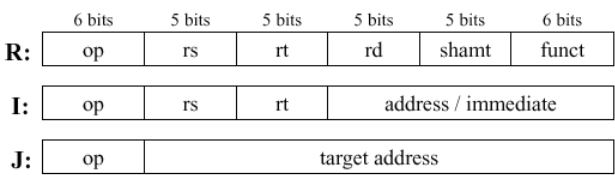
\includegraphics[scale=0.5]{figures/mips_instruction_types.png}
\caption{MIPS instruction types. Picture taken from http://www.cise.ufl.edu/~mssz/CompOrg/Figure2.7-MIPSinstrFmt.gif}
\label{fig:mips_instruction_types}
\end{figure}

The MIPS Instruction set is a Register-register type instruction set, and there are 32 registers listed in the MIPS Reference Data. The first register (register zero) always contains the value zero, and therefore this register is good for resetting values or to be used in logic operations. Then there are some reserved and non-reserved registers which can be used to hold values in words. Lastly the \$ra register (register 31) is the return address which is used when the jump and link (jal) function has to return.
Like all modern processor the MIPS-processor is Pipelined. There are five pipeline stages in the MIPS processor, the IF, ID, EX, MEM, WB. In the first stage the instruction is fetched (IF) from the memory and the program counter is increased by four bytes. Next is the decode stage (ID) where the right registers are read. In the execute stage the logic unit (ALU) calculates a result according to the instruction. The Memory stage is where the memory is accessed if needed in the instruction. In the write back stage (WB) the result of the ALU operation is put back in the right register.  
The MIPS processor optimizes performance by using branch prediction. This is a way of continue executing after a branch even though the result of the branch is not yet ready. This can either be done branch taken or the branch not taken terminology.
One of the forces of the MIPS processor is that it has a simple instruction set and a simple pipeline, these facts makes it easy to understand and program a MIPS computer. 

\subsubsection{The ARM architecture}
ARM (Advanced RISC Machine) is a 32-bit reduced instruction set computer (RISC) instruction set architecture (ISA). ARM has evolved over time, with the most recent revision defining three profiles: application, real-time and microcontroller. Each profile adds various instructions, so, in order to keep it simple, the following will consider the original implementation of ARM.
Originally ARM was hardwired without microcode in order to keep the design clean. It included the following RISC features:
\begin{itemize}
  \item Load/store architecture.
  \item No support for misaligned memory accesses.
  \item Uniform 16 × 32-bit register file.
  \item Fixed instruction width of 32 bits
  \item Mostly single-cycle execution.
  \end{itemize}
  Some additional design features were used to compensate for the simple design:
\begin{itemize}
  \item Conditional execution of most instructions in order to reduce branch overhead and compensate for the lack of a branch predictor.
  \item Arithmetic instructions only alter condition codes when desired.
  \item 32-bit barrel shifter which can be used without performance penalty with most arithmetic instructions and address calculations.
  \item Powerful indexed addressing modes.
  \item A link register for fast leaf function calls.
  \item Simple, but fast, 2-priority-level interrupt subsystem with switched register banks.
\end{itemize}
Newer revisions now have support for misaligned memory accesses, with some exceptions related to load/store multiple word instructions.
ARM has 37 Registers in total, all of which are 32-bits long. These are used as follows:
\begin{itemize}
  \item 1 dedicated program counter
  \item 1 dedicated current program status register
  \item 5 dedicated saved program status registers
  \item 30 general purpose registers
\end{itemize}
Earlier ARM implementations have a three stage pipeline, the stages being: fetch, decode and execute. Later designs have deeper pipelines for higher performance. The ARM processor used in iPhone 3GS has 13 stages. Other features and instructions have been developed to enhance performance, particularly the applications profile has been enhanced for multimedia performance.

\subsubsection{Conclusions}
Three widely used RISC architectures have been examined, ranging from the very simple PIC16 instruction set, to somewhat more advanced MIPS and ARM architectures. The simple instruction set of the PIC will allow for very simple, compact and power efficient implementation, but a lot of common operations (such as multiplication) are not available in the base instruction set. Furthermore, the accumulator type instructions mean, that a simple a = b + c instruction will have to be split up into multiple cycles, because at least one variable has to be in the accumulator register. The fact that all operations are based on byte-operands will also be a very limiting factor in a lot of common cases.
The somewhat more advanced 32-bit instruction word instruction sets of the MIPS and ARM architectures require a more complex hardware, but what they lack in simplicity, they make up for in versatility (obviously), and compared to more advanced CISC architectures (i.e. the Intel x86 family), they still retain all the advantages of simplicity.
